\documentclass{ximera}  

\title{Geometric Significance of Curl}  

\begin{document}  
\begin{abstract}  
%Geometry
\end{abstract}  
\maketitle 

Consider the vector field $\mathbf{F}(x,y)=(-y,0)$.

We can compute the curl of this vector field, 
\[
\nabla\times\mathbf{F}=(0,0,1)
\]

Imagine that we fix a point (representing a particle) in this vector field, but allow it to rotate. If imagine the vector field acting as a force on this particle, which way will it cause the particle to rotate?

(VECTOR FIELD)

Here, we see that the vector field is applying a greater force to the ``top'' of the particle than to the ``bottom.'' this will cause the particle to rotate counterclockwise. We describe this type of rotation as \emph{local rotation} or \emph{microscopic rotation}, since it's the rotation when we ``zoom in'' on the particle.

It turns out that the curl of a vector field provides a measure of this local rotation - but how are these connected? We will answer this question in this section, discussing the geometric significance of the curl.

\section{Geometric Significance of Two-dimensional Curl}

Recall that, for a two-dimensional vector field $\mathbf{F}(x,y)=(M,N)$, we can compute the curl as
\[
\nabla\times\mathbf{F} = (0,0,N_x-M_y)
\]
where $N_x$ is the partial derivative of $N$ with respect to $x$, and $M_y$ is the partial derivative of $M$ with respect to $y$. We'll start by considering how $M_y$ and $N_x$ contribute to local rotation.

First let's consider the case where $M_y<0$. In this case, the $x$-component of the vector field $\mathbf{F}$ is \emph{decreasing} as we move in the positive $y$ direction. Select all pictures which match this situation.

\begin{image}
\begin{tikzpicture}
\draw[->, very thick] (0,0) -- (2,0) ;
\draw[->, very thick] (.5,.5) -- (1.5,.5);
\node at (1, -1) {(a)};

\draw[->, very thick] (3,.5) -- (5,.5) ;
\draw[->, very thick] (3.5,0) -- (4.5,0);
\node at (4, -1) {(b)};

\draw[->, very thick] (7,0) -- (7,2) ;
\draw[->, very thick] (7.5,.5) -- (7.5,1.5);
\node at (7.25, -1) {(c)};

\draw[->, very thick] (10.5,0) -- (10.5,2) ;
\draw[->, very thick] (10,.5) -- (10,1.5);
\node at (10.25, -1) {(d)};

\draw[<-, very thick] (12,0) -- (14,0) ;
\draw[<-, very thick] (12.5,.5) -- (13.5,.5);
\node at (13, -1) {(e)};

\draw[<-, very thick] (15,.5) -- (17,.5) ;
\draw[<-, very thick] (15.5,0) -- (16.5,0);
\node at (16, -1) {(f)};

\draw[<-, very thick] (19,0) -- (19,2) ;
\draw[<-, very thick] (19.5,.5) -- (19.5,1.5);
\node at (19.25, -1) {(g)};

\draw[<-, very thick] (22.5,0) -- (22.5,2) ;
\draw[<-, very thick] (22,.5) -- (22,1.5);
\node at (22.25, -1) {(h)};
\end{tikzpicture}
\end{image}

\begin{selectAll}
\choice[correct] {(a)}
\choice {(b)}
\choice {(c)}
\choice {(d)}
\choice {(e)}
\choice[correct] {(f)}
\choice {(g)}
\choice {(h)}
\end{selectAll}

If $M_y<0$, which way will this cause a particle in the vector field to rotate?
\begin{multipleChoice}
\choice {Clockwise.}
\choice[correct] {Counterclockwise.}
\end{multipleChoice}

Now, let's consider the case where $N_x>0$. This means that the $y$-component of the vector field $\mathbf{F}$ is increasing as we move in the positive $x$ direction. Select all pictures which match this situation.

\begin{image}
\begin{tikzpicture}
\draw[->, very thick] (0,0) -- (2,0) ;
\draw[->, very thick] (.5,.5) -- (1.5,.5);
\node at (1, -1) {(a)};

\draw[->, very thick] (3,.5) -- (5,.5) ;
\draw[->, very thick] (3.5,0) -- (4.5,0);
\node at (4, -1) {(b)};

\draw[->, very thick] (7,0) -- (7,2) ;
\draw[->, very thick] (7.5,.5) -- (7.5,1.5);
\node at (7.25, -1) {(c)};

\draw[->, very thick] (10.5,0) -- (10.5,2) ;
\draw[->, very thick] (10,.5) -- (10,1.5);
\node at (10.25, -1) {(d)};

\draw[<-, very thick] (12,0) -- (14,0) ;
\draw[<-, very thick] (12.5,.5) -- (13.5,.5);
\node at (13, -1) {(e)};

\draw[<-, very thick] (15,.5) -- (17,.5) ;
\draw[<-, very thick] (15.5,0) -- (16.5,0);
\node at (16, -1) {(f)};

\draw[<-, very thick] (19,0) -- (19,2) ;
\draw[<-, very thick] (19.5,.5) -- (19.5,1.5);
\node at (19.25, -1) {(g)};

\draw[<-, very thick] (22.5,0) -- (22.5,2) ;
\draw[<-, very thick] (22,.5) -- (22,1.5);
\node at (22.25, -1) {(h)};
\end{tikzpicture}
\end{image}

\begin{selectAll}
\choice {(a)}
\choice {(b)}
\choice {(c)}
\choice[correct] {(d)}
\choice {(e)}
\choice {(f)}
\choice[correct] {(g)}
\choice {(h)}
\end{selectAll}

If $N_x<0$, which way will this cause a particle in the vector field to rotate?
\begin{multipleChoice}
\choice {Clockwise.}
\choice[correct] {Counterclockwise.}
\end{multipleChoice}

We've seen that the signs of $N_x$ and $M_y$ correspond to the direction of local rotation, with $N_x>0$ and $M_y<0$ contributing to counterclockwise rotation. 

In general, we have that the sign of $N_x-M_y$ corresponds to the direction of local rotation in the plane. In particular, we have the following correspondences:
\begin{align*}
N_x-M_y>0\;&\longleftrightarrow\; \textrm{counterclockwise local rotation}\\
N_x-M_y<0\;&\longleftrightarrow\; \textrm{clockwise local rotation}\\
N_x-M_y=0\;&\longleftrightarrow\; \textrm{no local rotation}\\
\end{align*}

Remembering that $N_x-M_y$ is the \emph{curl} of the two-dimensional vector field $\mathbf{F}$, we now have that the sign of the curl tells us the direction of local rotation for two-dimensional vector fields.

We have a special term for a vector field that never has any local rotation: we call such a vector field \emph{irrotational}.

Furthermore, the length of the curl,
\[
\|(0,0,N_x-M_y)\|=|N_x-M_y|,
\]
corresponds to the speed of rotation.

For example, in which case will the particle spin faster? 

\begin{multipleChoice}
\choice[correct]{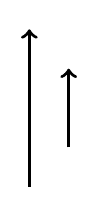
\begin{tikzpicture}
\draw[->, very thick] (0,0) -- (0,2) ;
\draw[->, very thick] (.5,.5) -- (.5,1.5);
\end{tikzpicture}}
\choice{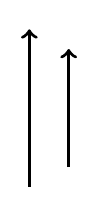
\begin{tikzpicture}
\draw[->, very thick] (0,0) -- (0,2) ;
\draw[->, very thick] (.5,.25) -- (.5,1.75);
\end{tikzpicture}}
\end{multipleChoice}

Note that this corresponds to a larger value of $N_x$ (the change in the $y$-component of $\mathbf{F}$ as we move in the positive $x$ direction).

We now apply our knowledge of the geometric significance of the curl in a couple of examples.

\begin{example}
Consider the vector field $\mathbf{F}(x,y)=(-y,x^2)$. Compute the curl of $\mathbf{F}$, and describe the local rotation of the vector field at the points $(1,0)$ and $(-4,1)$.
\begin{explanation}
We begin by computing the curl of $\mathbf{F}$,
\[
\nabla\times\mathbf{F} = (0,0,\answer{2x+1}).
\]
At the point $(1,0)$, we have $(\nabla\times\mathbf{F})(1,0) = (0,0,\answer{3})$. Looking at the third component, we see that the sign of $N_x-M_y$ at $(1,0)$ is \wordChoice{\choice[correct]{positive}\choice{negative}\choice{zero}}. Thus, the local rotation of the vector field at the point $(1,0)$ is \wordChoice{\choice{clockwise}\choice[correct]{counterclockwise}\choice{no rotation}}.

At the point $(-4,1)$, we have $(\nabla\times\mathbf{F})(1,0) = (0,0,\answer{7})$. Looking at the third component, we see that the sign of $N_x-M_y$ at $(-4,1)$ is \wordChoice{\choice{positive}\choice[correct]{negative}\choice{zero}}. Thus, the local rotation of the vector field at the point $(-4,1)$ is \wordChoice{\choice{clockwise}\choice[correct]{counterclockwise}\choice{no rotation}}.

Looking at a graph of the vector field, we can see that this local rotation is reflected in the graph.

(ADD GRAPH, WITH ROTATION?)
\end{explanation}
\end{example}

\begin{example}
Let $\mathbf{F}(x,y)=\left(\dfrac{y}{x^2+y^2},\dfrac{x}{x^2+y^2}\right)$. Compute the curl $\nabla\times\mathbf{F}$, and interpret it geometrically.
\begin{explanation}
Computing our partial derivatives, we have
\[
N_x = \answer{\frac{x^2+y^2-2x^2}{(x^2+y^2)^2}}
\]
and 
\[
M_y = \answer{\frac{-x^2-y^2+2x^2}{(x^2+y^2)^2}}.
\]
Then, the curl of $\mathbf{F}$ is
\[
\nabla\times\mathbf{F} = (0,0,\answer{0}).
\]

Thus, we see that there is no local rotation at any point in the vector field. This is particularly interesting once we look at a graph of the vector field.

(GRAPH)

From the graph of the vector field, there certainly seems to be some larger scale, global rotation of the vector field. However, our computation showed that there is no local rotation. This example illustrates an important distinction: curl measures \emph{local} rotation of a vector field, which is a different concept from \emph{global} rotation.
\end{explanation}
\end{example}

In this section, we saw how the curl of a vector field corresponded to local rotation for a two-dimensional vector field. In the next section, we describe how the curl of a vector field corresponds to local rotation for \emph{three}-dimensional vector fields.

\section{Geometric Significance of Three-dimensional Curl}

For a three dimensional vector field $\mathbf{F}(x,y,z)=(M,N,P)$, we can compute the curl of $\mathbf{F}$ as
\[
\nabla\times \mathbf{F} = (P_y-N_z, \answer{-P_x+M_z},\answer{N_x-M_y}).
\]
Here, the situation is more complicated than in two dimensions. In the plane, there are only two possible ways to rotate: clockwise and counterclockwise. In $\mathbb{R}^3$, there are infinitely many different ways to rotate, since we have infinitely many choices of axes. Yikes!

Fortunately, three-dimensional curl still tells about local rotation. In this case, we imagine local rotation as rotation of an infinitesimal (tiny) sphere. This sphere can rotate in infinitely many different ways, depending on which axis we rotate around.

When we look at the components of the curl, this tells us about rotation perpendicular to each of the axes, ignoring rotation in any other direction. Specifically,
\begin{align*}
N_x-M_y\textrm{ (the $z$-component of $\mathbf{F}$)}\;&\longleftrightarrow\;\textrm{ rotation perpendicular to the $z$-axis)}\\
P_y-N_z\textrm{ (the $x$-component of $\mathbf{F}$)}\;&\longleftrightarrow\;\textrm{ rotation perpendicular to the $x$-axis)}\\
-P_x+M_z\textrm{ (the $y$-component of $\mathbf{F}$)}\;&\longleftrightarrow\;\textrm{ rotation perpendicular to the $y$-axis)}
\end{align*}

Once again, the sign tells us the direction of rotation, with positive sign corresponding to counterclockwise rotation (viewed from the positive axes).

Furthermore, the length of the curl, $\|\nabla\times\mathbf{F}\|$, tells us the speed of rotation, and the direction of $\nabla\times\mathbf{F}$ tells us the axis of rotation.

In $\mathbb{R}^3$, we would like to be able to describe the direction of rotation around a given axis. However, this can be tricky, since it's a matter of perspective. Imagine rotation in the $xy$-plane. If the rotation is clockwise viewed from above, then it will be counterclockwise from below! Fortunately, curl follows the \emph{right hand rule}:
\begin{itemize}
\item[] If you point your right thumb in the direct of $\nabla\times\mathbf{F}$, then your fingers will curl in the direction of local rotation.
\end{itemize}

We now put this to use in an example.

\begin{problem}
Consider the vector field $\mathbf{F}(x,y,z)=\left(0,\dfrac{-z}{(y^2+z^2)^{3/2}},\dfrac{y}{(y^2+z^2)^{3/2}}\right)$. Compute the curl of $\mathbf{F}$.
\[
\nabla\times\mathbf{F} = \answer{(\frac{-1}{(y^2+z^2)^{3/2}},0,0)}
\]
\begin{problem}
What is the axis of local rotation (at any point)?
\begin{multipleChoice}
\choice[correct] {The $x$-axis.}
\choice {The $y$-axis.}
\choice {The $z$-axis.}
\choice {Some other line.}
\end{multipleChoice}
\begin{problem}
Viewed from the positive $x$-axis, what is the direction of local rotation (at any point)?
\begin{multipleChoice}
\choice[correct] {Clockwise.}
\choice {Counterclockwise.}
\end{multipleChoice}
\begin{problem}
How does the speed of local rotation change as we move closer to the origin?
\begin{multipleChoice}
\choice {Stays the same.}
\choice {Gets slower.}
\choice[correct] {Gets faster.}
\end{multipleChoice}
\end{problem}
\end{problem}
\end{problem}
\end{problem}

We've now seen how the curl describes the local rotation of a three-dimensional vector field. In the next section, we'll cover some connections of the curl to previous topics.

\section{Summary}

In this section, we studied the geometric significance of the curl. We found that the curl gives a measure of the local rotation of a vector field.

For a two-dimensional vector field, the sign of the curl told us the direction of rotation. Specifically, we have the following correspondence.
\begin{align*}
N_x-M_y>0\;&\longleftrightarrow\; \textrm{counterclockwise local rotation}\\
N_x-M_y<0\;&\longleftrightarrow\; \textrm{clockwise local rotation}\\
N_x-M_y=0\;&\longleftrightarrow\; \textrm{no local rotation}\\
\end{align*}
The magnitude $|N_x-M_y|$ corresponds to speed of rotation.

For a three-dimensional vector field, the components of the curl tell us about local rotation perpendicular to the axes. We also have:
\begin{itemize}
\item The length of the curl, $\|\nabla\times\mathbf{F}\|$, corresponds to the speed of rotation.
\item The direction of the curl vector $\nabla\times\mathbf{F}$ gives the axis of rotation.
\item Curl follows the right hand rule: if you point your thumb in the direction of $\nabla\times\mathbf{F}$, your fingers curl in the direction of local rotation.
\end{itemize}

In the next section, we'll consider the curl of a conservative vector field, and how the curl connects to Green's Theorem.

\end{document}